
%(BEGIN_QUESTION)
% Copyright 2012, Tony R. Kuphaldt, released under the Creative Commons Attribution License (v 1.0)
% This means you may do almost anything with this work of mine, so long as you give me proper credit

A house has a 3:12 roof slope.  Supposing that one of the triangular truss structures in the roof bears 500 pounds of snow load (equivalent to 500 pounds of force applied to the peak of the triangle), how much tensile (pulling) force will there be in the horizontal beam?

$$\includegraphics[width=15.5cm]{i02577x01.eps}$$

$F_{beam}$ = \underbar{\hskip 50pt} lbs

\vskip 10pt

\underbar{file i02577}
%(END_QUESTION)





%(BEGIN_ANSWER)

It might be easier to approach this problem if we consider one-half of the truss at a time.  The 500 pounds snow load will be evenly borne by each side of the truss, such that the tension in each half of the horizontal beam handles half of the force necessary to create the 500 pounds of upward force resisting the snow.  

Our pitch ratio of 3:12 (or 1:4) tells us the horizontal beam tension will be four times the snow load.  If each half of the truss bears 250 pounds of snow, then each half of the horizontal beam will experience 1000 pounds of tension.  The two beam halves' tensions translate into 250 pounds of vertical force (each), making 500 pounds of vertical force.  The 1000 pounds of tension in each half of the beam do {\it not} add up to 2000 pounds because the tension in each beam half is pointed in opposite directions in order for the horizontal forces to cancel (otherwise, the truss would be accelerating horizontally!):

$$\includegraphics[width=15.5cm]{i02577x02.eps}$$

%(END_ANSWER)





%(BEGIN_NOTES)


%INDEX% Mathematics review: trigonometric calculations

%(END_NOTES)


